\section{Analysis} \label{sec:Analysis}

\subsubsection{Calibrated Model}

\begin{table}[H]
\begin{adjustbox}{max width=\textwidth}
\begin{threeparttable}[b]
\caption{Parameters of the model}
\label{tab:ModelCalib}
\begin{tabular}{@{}lllcc@{}}
\toprule
 & Parameter                              & Notation         & Calibration & \citet{Campbell1999}\\ \midrule 
\multicolumn{5}{l}{\textit{Calibrated}}                                    \\
 & Mean consumption growth                & $g$              & $0.0134$  & $0.0189$\\
 & Standard deviation of $\Delta c_t$     & $\sigma$         & $0.0152$  & $0.0150$\\
 & Standard deviation of $\Delta d_t$     & $\sigma_w$       & $0.1256$  & $0.1120$\\
 & Log risk-free rate                     & $r^f$            & $0.0109$  & $0.0094$\\
 & Persistence parameter                  & $\phi$           & $0.9008$  & $0.8700$\\
 \multicolumn{5}{l}{\textit{Assumed}}                                      \\
 & Coefficient of Risk Aversion           & $\gamma$         & $2.0000$  & $2.0000$\\
 & Correlation dividends/consumption      & $\rho$           & $0.2000$  & $0.2000$\\
\multicolumn{5}{l}{\textit{Implied}}                                       \\
 & Subjective discount factor             & $\delta$         & $0.9156$  & $0.8900$\\
 & Steady-state surplus consumption ratio & $\Bar{S}$        & $0.0666$  & $0.5700$\\
 & Maximum surplus consumption ratio      & $S_{\text{max}}$ & $0.1096$  & $0.0940$\\ \bottomrule
\end{tabular}
\begin{tablenotes}
\footnotesize{\item [1] All relevant parameters are annualized
              \item [2] Calibrated parameters are estimated from data, assumed are chosen arbitrarily on the grounds of existing literature, while implied parameters are calculated from the calibrated/assumed parameters.}
\end{tablenotes}
\end{threeparttable}
\end{adjustbox}
\end{table}


Compared to the calibration of \citet{Campbell1999}, our calibration suggests a higher persistence parameter, higher volatility of dividend growth and lower consumption growth, the implied surplus consumption parameters suggests a slightly higher overall surplus consumption. The differences likely stems from the extra 20 years of calibration data. \\

\subsection{Simulation}
From the calibrated model we simulate a chain of 100.000 monthly draws from the economy yielding 8.332 years of simulated time-series. We find in addition to the series that the procedure is extremely sensitive to the distribution of grid points. We use 10 equally distributed grid-points and an additional 6 just below $s_max$.

\begin{table}[H]
\centering
\caption{Simulated Moments}
\label{tab:simmom}
\begin{tabular}{@{}lllll@{}}
\toprule
Statistic                                               & \makecell{Consumption \\ Claim} & \makecell{Dividend \\ Claim} & \makecell{CC99-Calibration \\ Consumption Claim} & \makecell{CC99-Calibration\\ Dividend Claim} \\ \midrule
$\mathbb{E}\left(\Delta c \right)$                      &0.013504&0.011661&0.019024&0.017369\\
$\sigma\left(\Delta c \right)$                          &0.01243&0.10257&0.012268&0.09147\\
$\mathbb{E}r^f$                                         &0.010881&0.010881&0.0094&0.0094\\
$\mathbb{E}\left(r-f^f\right)/\sigma\left(r-r^f\right)$ &0.37625&0.23074& 0.43644                                       &         0.31764                            \\
$\mathbb{E}\left(R-R^f\right)/\sigma\left(R-R^f\right)$ & 0.4173   & 0.31102               &  0.4761                                      &      0.389                               \\
$\mathbb{E}\left(r-r^f\right)$                          &  0.048783                 &      0.045342          &         0.067377                               &        0.06472                             \\
$\sigma\left(r-r^f\right)$                              &     0.12965              &       0.19651           &   0.15438                                       &                  0.19651                     \\
$\mathbb{E}\left(p-c\right)$                          &     3.1123                &      3.157            &         2.8926                                 &             2.9161                          \\
$\sigma\left(p-c\right)$                              &       0.26201            &      0.28973          &   0.27676                                     & 0.29361                                    \\ \bottomrule
\end{tabular}
\end{table}



Allowing us to infer about the predictability of excess stock returns, during times of simulated crisis. 
\newline
\\
Based on NCER-recession data, we find that the US economy was in recession approximately 13.4\% of the period spanning January 1950 until December 2018.  In the model a recession implies that present consumption in low relative to previous periods consumption, that is the value of $s_t$ is lower than the steady state value of surplus consumption $\Bar{s}$ - integrating over the density of $s_t$ yields that the simulated economy is in recession during 37\% of all observations, which indicates that $\Bar{s}$ might be misspecified. To correct $\Bar{s}$ we match the empirical business cycle behavior by numerical optimization of the $s_t$ density, such that the empirical and simulated economy is in recession roughly the same amount. The $\Bar{s}$-value matching the empirical business cycle, throughout denoted $\Bar{s}_{rec}$ \textit{or} ($\Bar{S}_{rec}$), is found to be $-3.18$ ($0.0415$). One additional recessions specification we denote as $\bar{s}_{2,rec}$ is chosen as to capture only the most extreme non-linearity of the relationship between surplus consumption and expected returns as presented in figure \ref{fig:SPCPD-a}.

\begin{table}[H] 
\centering
\caption{Business Cycle, Simulated and historic}
\label{tab:BC}
\begin{tabular}{@{\hspace{8mm}}ll@{\hspace{5mm}}ccc@{}}
\toprule
                       & \multicolumn{3}{c}{\textit{Simulated}} & \textit{Historic}  \\ \midrule
                                          & $\Bar{S}$       & $\Bar{S}_{REC}$ & $\Bar{S}_{2,REC}$&    \\ \cmidrule(l){2-4} 
        \textit{Value}                        & 0.067 & 0.042& 0.02 &              \\
Recession,                                      \% &36.92 & 13.41 &2.83  & 13.41\\ \bottomrule
\end{tabular}
\end{table}




\begin{figure}[H]
    \centering
    \caption{Distribution of simulated $s_t$ chain}
    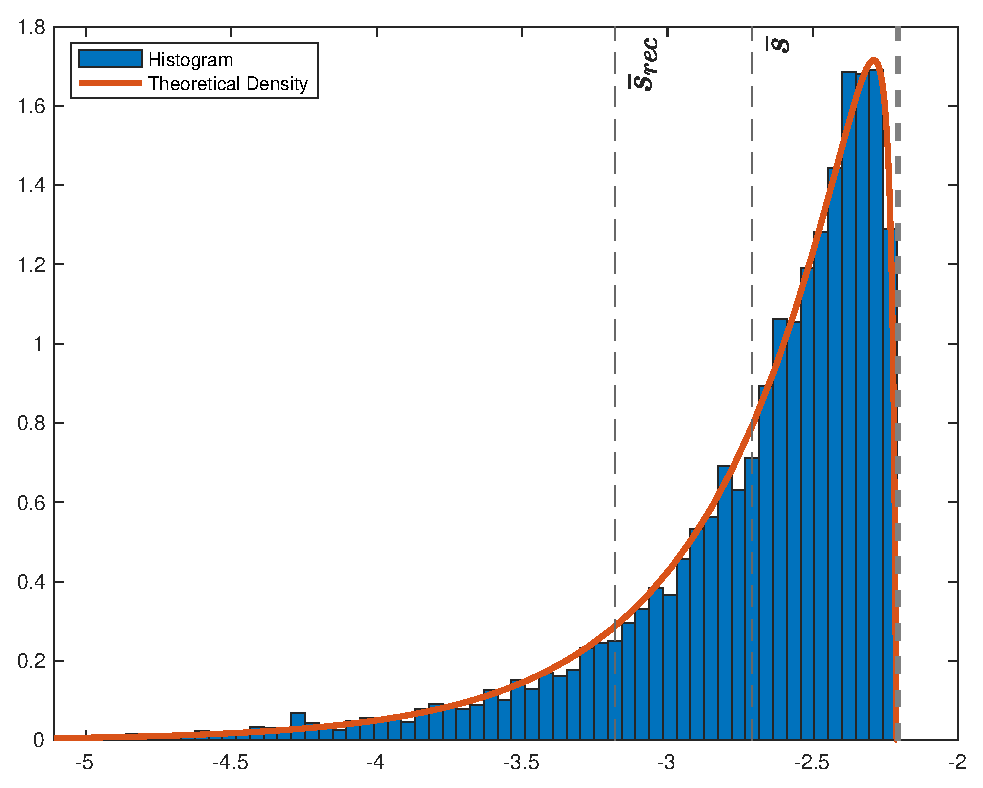
\includegraphics[width=\textwidth]{Figures/DistributionS_t.eps}
    \label{fig:DistriSt}
\end{figure}
From the constructed surplus consumption threshold $\Bar{s}_{rec}$ for recession, we construct an indicator dummy for recessions. Such that $I_{rec} = 1$ \textit{iff}. $\Bar{s}_{rec} > s_t$ and $I_{rec}=0$ otherwise.

Having simulated an economy based upon habit formation, and justified our choice of recession periods of the simulated series, we are able to test the proposed hypothesis:
\begin{enumerate}
    \item Is the model of \citet{Campbell1999} able to generate returns with the following two properties
    \begin{enumerate}
        \item Returns are predictable by the price/consumption- or the price/dividend-ratio under recessionary periods?
        \item Returns are unpredictable by the price/consumption- or the price/dividend-ratio under expansionary periods?
    \end{enumerate}
\end{enumerate}
Examining the expected returns as a function of the surplus consumption ratio, as in figure \ref{fig:SPCPD-a}. The model reveals a somewhat linear relationship for high values of the surplus consumption, the relationship however is much more steep and nonlinear when $S_t$ approaches ${S}_{REC}$, the goal is then to exploit this fact when predicting returns.


\begin{comment}
\begin{figure}[H]
    \centering
    \caption{Expected returns as a function of $S_t$}
    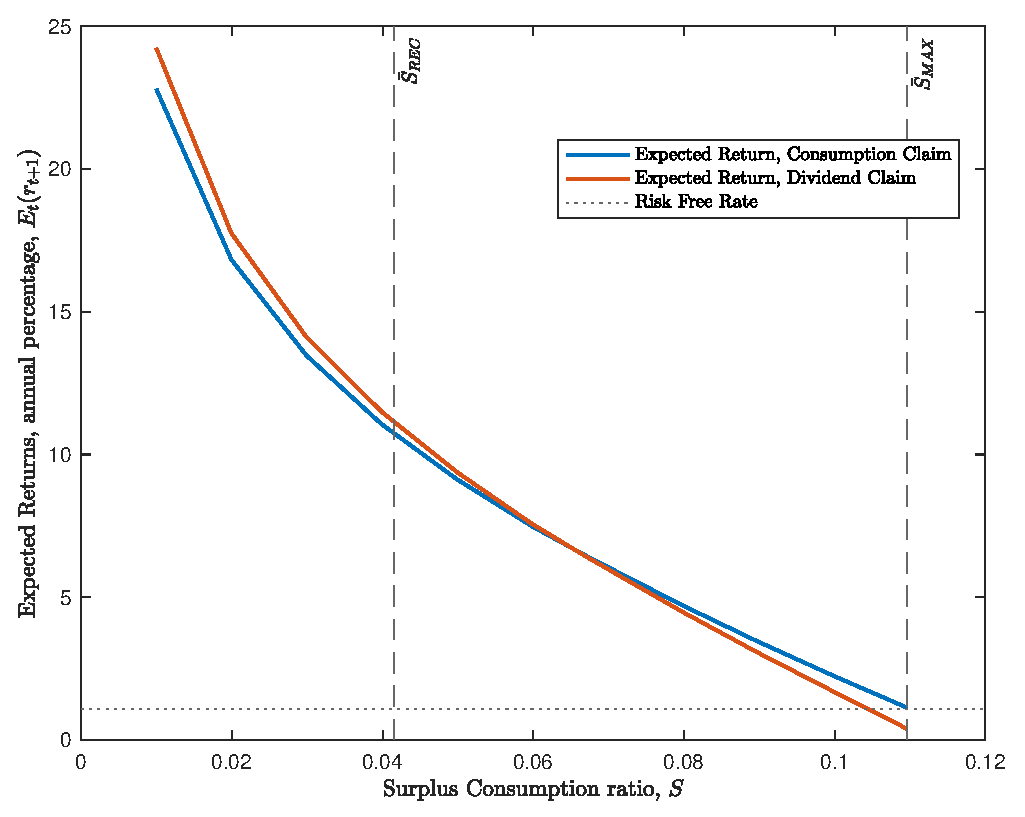
\includegraphics{Figures/ErPCPD.eps}
    \label{fig:ErPCPD}
\end{figure}
\end{comment}


\begin{figure}[H]
\centering
\caption{Functionals of surplus consumption ratio}
    \label{fig:SPCPD}
\subfigure[Expected returns as a function of $S_t$]{\label{fig:SPCPD-a}
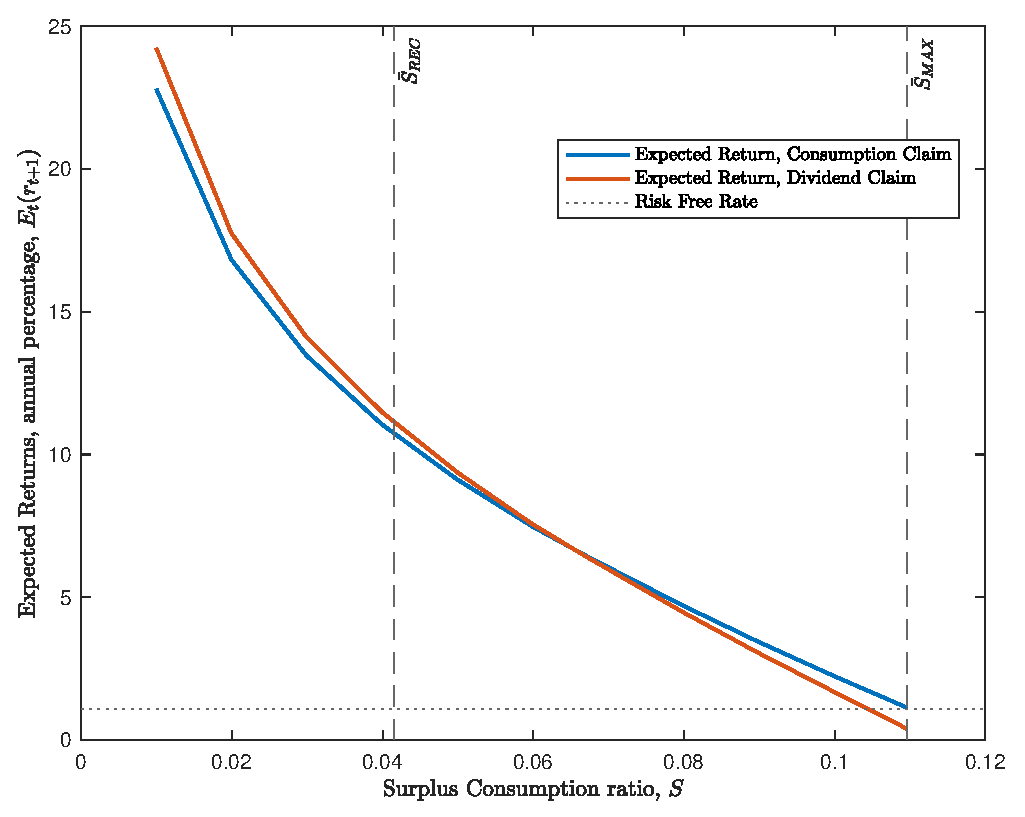
\includegraphics[width=0.45\textwidth]{Figures/ErPCPD.eps}} ~
\subfigure[$P/C$, $P/D$ as a function of $S_t$]{
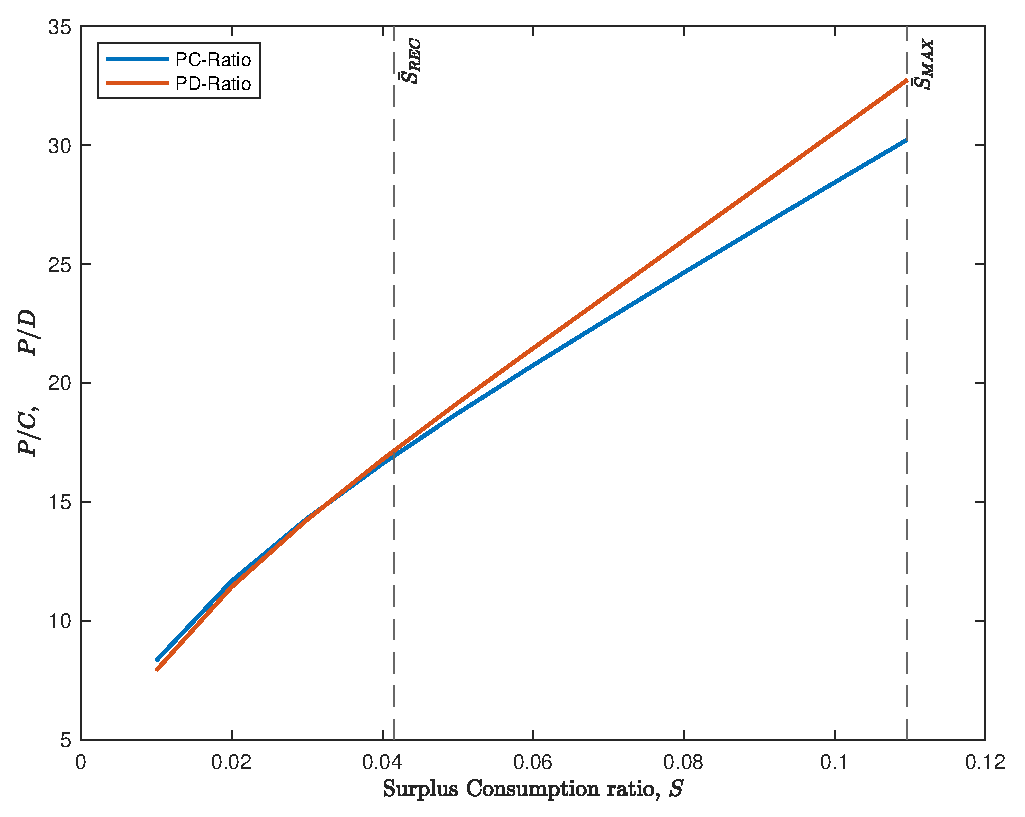
\includegraphics[width=0.45\textwidth]{Figures/PC_PD_Ratio.eps}}
\end{figure}

From the functionals of surplus consumption ratio reported in \ref{fig:SPCPD}, some basic predictions can be made. We see that when surplus consumption is low, that is in recessionary times, expected returns increases, the intuition is that when times are bad, as consumption falls relative to habit levels, the risk aversion increases, people wants a higher level of compensation per unit of risk - the risk premium rises - note that this must hold true for all levels of $S$ as the risk-free rate is fixed in the model. \\
Furthermore the figure implies that the regression coefficient of $P/C$ or equivalent $P/D$ should be negative. Lower P/C or P/D implies higher values of $\mathbb{E}\left[r_t-r^f\right]$, both driven by the single state. 


\subsection{Results}
First we estimate the following regressions:
\begin{align*}
     r_{t+1} - r^{f} &= \alpha + \beta_{REC} \left( p_t - c_t \right) * I_{t,REC} + \beta_{EXP} \left( p_t - c_t \right) * \left(1 - I_{t,REC}\right)  + \varepsilon_{t+1}\\
      r_{t+1} - r^{f} &= \alpha + \beta_{REC} \left( p_t - d_t \right) * I_{t,REC} + \beta_{EXP} \left( p_t - d_t \right) * \left(1 - I_{t,REC}\right)  + \varepsilon_{t+1}\\
      r_{t+1} - r^{f} &= \left(\alpha_{REC} + \beta_{REC} \left(p_t - c_t\right)\right)*I_{REC} + \left(1-I_{REC}\right) \left( \alpha_{EXP} + \beta_{EXP}\left(p_t - c_t \right) \right) + \varepsilon_{t+1}\\
r_{t+1} - r^{f} &= \left(\alpha_{REC} + \beta_{REC} \left(p_t - d_t\right)\right)*I_{REC} + \left(1-I_{REC}\right) \left( \alpha_{EXP} + \beta_{EXP}\left(p_t - d_t \right) \right) + \varepsilon_{t+1}      
\end{align*}
That is we use the recession indicator to infer the influence of the predictors in respectively recessions and expansions.\\
As a benchmark we run two additional regressions given:
\begin{align*}
     r_{t+1} - r^{f} &= \alpha + \beta \left( p_t - c_t \right)  + \varepsilon_{t+1}\\
      r_{t+1} - r^{f} &= \alpha + \beta \left( p_t - d_t \right) + \varepsilon_{t+1}
\end{align*}
Figure \ref{tab:regress1} reports results of the four regressions. The desired property of separability of business cycles does not get a lot of support from this exact result. We see no increase in $R^2$, we find strong statistical evidence supporting rejection of the null-hypothesis for all estimates in all four regressions, this is however to be expected as the sample size of 8331 observations is quite large, it is well established that as the sample size increases the asymptotic variance of the OLS-estimate decreases and thus significance is inevitable as the sample size becomes quite large.
\begin{table}[H]
\centering   
  \caption{Regressions, $\Bar{S}_{REC} = 0.041542$}           
  \label{tab:regress1}     
  \begin{threeparttable}
\begin{tabular}{@{\hspace{5pt}}l@{\hspace{5pt}}cccccc} 
\toprule 
 & \multicolumn{6}{c}{\textit{Dependent variable:}} \\ 
 & \multicolumn{6}{c}{$\left(r_{t+1}-r^f\right)$} \\ 
 \cmidrule(rr){2-7}
 & (1) & (2) & (3) & (4) & (5) & (6) \\ 
\midrule  
\\[-2.1ex] $\left( p_t - c_t \right)_{REC}$ &-0.169& &0.03228 & & &\\ 
  & (0.012) & &(0.0023) & & & \\ 
 \addlinespace 
  $\left( p_t - c_t \right)_{EXP}$ &-0.1641  &    & &-0.02975 & &  \\ 
  & (0.0098) & & &(0.0019) & & \\ 
 \addlinespace 
  $\left( p_t - d_t \right)_{REC}$ & &-0.1719& & & 0.03658  &   \\ 
                                   & &  (0.016) & & & (0.0031) &    \\ 
 \addlinespace 
  $\left( p_t - d_t \right)_{EXP}$ & &   -0.1668& & & &-0.03338 \\ 
                                   & &  (0.012) & & & &(0.0024) \\ 
 \addlinespace 
 Constant &0.5611 &0.5736&0.03789 &0.1313 &0.03305 &0.1395 \\ 
          &(0.032) &(0.041)&(0.0013)&(0.0059)&(0.0021)&(0.0077) \\ 
 \addlinespace 
\midrule  
Observations & 8331 & 8331&8331 & 8331&8331&8331\\
R$^{2}$ &0.094 & 0.053&0.047&0.062&0.026&0.035 \\ 
Residual Std. Error &0.015 & 0.037&0.016&0.016&0.038&0.037 \\ 
\bottomrule 
\end{tabular} 
\begin{tablenotes}
\footnotesize{
\item[1] Brackets below estimates contains Newey-West corrected standard errors. 
\item[2] Regressions on 8331 years of simulated data.
\item[3] EXP (REC) denotes expansion (recession)
}
\end{tablenotes}
\end{threeparttable}
\end{table} 


However from figure \ref{fig:SPCPD-a} we see that the most extreme effect of $S_t$ on expected returns kicks in at an estimated $0.02$, based on this fact we run additional regressions with the same specification as above, where we respecify $\Bar{S}_{REC}=0.02$, the output of which is reported in table \ref{tab:regress2}. This specification of $\Bar{S}_{REC}$ implies that the simulated economy is in recession approximately 2.8\% of the time.

\begin{table}[H]
\centering   
  \caption{Benchmark regressions}           
  \label{tab:regress1}     
  \begin{threeparttable}
\begin{tabular}{@{\hspace{5pt}}l@{\hspace{15pt}}c@{\hspace{5pt}}c} 
\toprule 
 & \multicolumn{2}{c}{\textit{Dependent variable:}} \\ 
 & \multicolumn{2}{c}{$\left(r_{t+1}-r^f\right)$} \\ 
 \cmidrule(rr){2-3}
 & (1) & (2)\\ 
\midrule  
\\[-2.1ex] $ p_t - c_t $ &-0.1516&\\ 
  & (0.0071) &  \\ 
 \addlinespace 
  $p_t - d_t $ & &   -0.137 \\ 
               & &  (0.0064) \\ 
 \addlinespace 
 Constant &0.5206 &0.4814\\ 
          &(0.023) &(0.021) \\ 
 \addlinespace 
\midrule  
Observations & 8331 & 8331\\
R$^{2}$ &0.094 & 0.094 \\ 
Residual Std. Error &0.015 & 0.015 \\ 
\bottomrule 
\end{tabular} 
\begin{tablenotes}
\footnotesize{
\item[1] Brackets below estimates contains Newey-West corrected standard errors. 
\item[2] Regressions on 8331 years of simulated data.
\item[3] EXP (REC) denotes expansion (recession)
}
\end{tablenotes}
\end{threeparttable}
\end{table} 


\begin{table}[H]
\centering   
  \caption{Regressions}           
  \label{tab:regress2}     
  \begin{threeparttable}
\begin{tabular}{@{\hspace{5pt}}l@{\hspace{5pt}}cccccc} 
\toprule 
 & \multicolumn{6}{c}{\textit{Dependent variable:}} \\ 
 & \multicolumn{6}{c}{$\left(r_{t+1}-r^f\right)$} \\ 
 \cmidrule(rr){2-7}
 & (1) & (2) & (3) & (4) & (5) & (6) \\ 
\midrule  
\\[-2.1ex] $\left( p_t - c_t \right)_{REC}$ &-0.1353& &0.06422 & & &\\ 
  & (0.013) & &(0.0056) & & & \\ 
 \addlinespace 
  $\left( p_t - c_t \right)_{EXP}$ &-0.1439  &     &-0.05878 & &  \\ 
  & (0.0081) & &(0.0037) & & \\ 
 \addlinespace 
  $\left( p_t - d_t \right)_{REC}$ & &-0.1205& & & & 0.06511  &   \\ 
                                   & &  (0.012) & & & & (0.0057) &    \\ 
 \addlinespace 
  $\left( p_t - d_t \right)_{EXP}$ & &   -0.1297& & & & &-0.05811 \\ 
                                   & &  (0.0073) & & & & &(0.0036) \\ 
 \addlinespace 
 Constant &0.4959 &0.4576&0.0441 &0.2274 &0.04412 &0.2281 \\ 
          &(0.026) &(0.024)&(0.0014)&(0.012)&(0.0014)&(0.012) \\ 
 \addlinespace 
\midrule  
Observations & 8331 & 8331& 8331&8331&8331\\
R$^{2}$ &0.094 & 0.094&0.039&0.072&0.039&0.074 \\ 
Residual Std. Error &0.015 & 0.015&0.016&0.016&0.016&0.016 \\ 
\bottomrule 
\end{tabular} 
\begin{tablenotes}
\footnotesize{
\item[1] Brackets below estimates contains Newey-West corrected standard errors. 
\item[2] Regressions on 8331 years of simulated data.
\item[3] EXP (REC) denotes expansion (recession)
}
\end{tablenotes}
\end{threeparttable}
\end{table} 


\begin{table}[H]
    \centering
    \caption{Long Run Regressions}
   \begin{tabular}{l@{\hspace{8mm}}cccc}
   \toprule
\textit{Horizon, Years}& $\beta_{pc}$ & $R^2_{pc}$ & $\beta_{pd}$ & $R^2_{pd}$ \\ 
\midrule
1 & -0.135 & 0.0736 & -0.122 & 0.0735 \\ 
2 & -0.273 & 0.1574 & -0.247 & 0.1572 \\ 
3 & -0.398 & 0.2324 & -0.360 & 0.2321 \\ 
5 & -0.617 & 0.3580 & -0.558 & 0.3576 \\ 
7 & -0.790 & 0.4525 & -0.714 & 0.4521 \\ 
10 & -0.979 & 0.5492 & -0.885 & 0.5488 \\ 
\bottomrule 
\end{tabular}
    \label{tab:LHREGRESSION}
\end{table}

\begin{comment}
\midrule
1 & -0.13493 & 0.073631 & -0.12195 & 0.073542 \\ 
2 & -0.27306 & 0.15742 & -0.2468 & 0.15724 \\ 
3 & -0.39824 & 0.23238 & -0.35995 & 0.23213 \\ 
5 & -0.61689 & 0.35796 & -0.55757 & 0.35757 \\ 
7 & -0.78972 & 0.45245 & -0.71386 & 0.45206 \\ 
10 & -0.9792 & 0.54915 & -0.88524 & 0.5488 \\ 
\bottomrule 
\end{comment}

Instead we run a regime-switching linear regression with observable states, remember that from the simulation we obtained the surplus consumption ratio as an observable. In real data one would have to rely on latent state regressions such as a \textit{hidden Markov model}, to determine the latent state as a function of $s_t$.\\
However we have the simulated series and are able to run the regression straightforward. We run four regressions again with excess stock return as the regressand:

\begin{align*}
    \left(r_{t+1} - r^{f}\right) I_{t+1,REC} &=  \alpha + \beta \left( p_t - c_t \right) I_{REC,t} + \varepsilon_{t+1}\\
    \left(r_{t+1} - r^{f}\right)I_{t+1,REC} &=  \alpha + \beta \left( p_t - d_t \right) I_{REC,t} + \varepsilon_{t+1}\\
    \left(r_{t+1} - r^{f}\right)I_{t+1,EXP} &=  \alpha + \beta \left( p_t - c_t \right) \left( 1- I_{REC,t}\right)  + \varepsilon_{t+1}\\
    \left(r_{t+1} - r^{f}\right)I_{t+1,EXP} &=  \alpha + \beta \left( p_t - d_t \right) \left( 1- I_{REC,t}\right) x+ \varepsilon_{t+1}
\end{align*}

The results of the four regressions are reported in table \ref{tab:RSregress}, the results are quite interesting. Examining the results reveals that with a regime switching approach as opposed to the previous single state regression, we are able to split the effects of business cycles on the predictability of stock returns. Notice how the coefficients indicating the effects of respectively P/C and P/D ratios on excess returns have switched signs in recession periods, while the constant effect is negative during recessions, indicating the base effect of being in a recession on excess returns is negative. However while not intuitively inappropriate in this context it have to be noted that expected returns are restricted to be positive in this model, therefore mandating that the size of the log P/C and log P/D-ratios must be large enough to offset the negative constant. This restriction is not particular restrictive as the log price consumption-ratio and equivalent log price dividend ratio is seldom below 2, see the simulated chains of log P/C and log P/D in figure \ref{fig:PCPD} in appendix.\\

Another result worth noting is one that provides evidence in favor of both of our hypothesis, that is the estimated coefficient of determination is much higher in the recession periods reaching 7\% when predicting excess returns using the price-consumption-ratio, than it is in expansionary periods reaching just barely .2\%, using the price-dividend-ratio as the predictor yields a smaller $R^2$ this is to be expected, as the price-dividend is by construction a noisier mapping of the price-consumption-ratio dynamics, containing not only the shock to consumption growth $\sigma$ but also the shock to dividend growth $\sigma_w$.\\

Now in real data it is not plausible to condition the regressand on a future variable like we do with the recession indicator. The reason why it is still not completely unreasonable is the high persistence of $s_t$, remember that $s_t$ is driven by the highly persistent growth rate of consumption, estimating the persistence in our simulation yields an autocorrelation coefficient of $0.9972$.\\
In real data it would be more reasonable to estimate a transition probability matrix to forecast the underlying business cycle chain, and condition on the recession forecast. Recession forecasts, however, are notoriously unreliable, comtaminating the estimates with very high levels of uncertainty.


\begin{table}[H]
\centering   
  \caption{Regime Switching Regression}           
  \label{tab:RSregress}     
  \begin{threeparttable}
\begin{tabular}{@{\hspace{5pt}}l@{\hspace{5pt}}cccc} 
\toprule 
 & \multicolumn{4}{c}{\textit{Dependent variable:}} \\ 
 & \multicolumn{2}{c}{$\left(r_{t+1}-r^f\right)_{REC}$} & \multicolumn{2}{c}{$\left(r_{t+1}-r^f\right)_{EXP}$} \\ 
 \cmidrule(rr){2-5}
 & (1)   &   (2) & (3) & (4) \\ 
\midrule  
\\[-2.1ex] $ p_t - c_t $ & 0.001174&  &-0.0003139   & \\ 
  & (9.4e-05) & &(3.6e-05) & \\ 
 \addlinespace 
 $p_t - d_t$ &  & 0.001168 & &-0.000323 \\
 & & (9.4e-05) & &(3.523e-05) \\
 \addlinespace 
 Constant &-0.0005367 &-0.0005311 &0.00537 &0.005429 \\ 
  &(2.3e-05) &(2.3e-05) &(0.00018) &(0.00018) \\ 
 \addlinespace 
\midrule  
Observations & 99999 & 99999 & 99999 &99999\\ 
R$^{2}$ &0.009 & 0.0089 & 0.00036 &0.00039\\ 
Residual Std. Error &0.00045 & 0.00045 &0.001 & 0.001  \\ 
\bottomrule 
\end{tabular} 
\begin{tablenotes}
\footnotesize{
\item[1] Brackets below estimates contains \citet{NW87} corrected standard errors. 
\item[2] Regressions on 99999 months of simulated data.
\item[3] EXP (REC) denotes expansion (recession)
}
\end{tablenotes}
\end{threeparttable}
\end{table} 



\begin{comment}
\begin{table}[H]
\centering
\caption{Simulated Moments}
\label{tab:MMoomme}
\begin{tabular}{@{}llllllllll@{}}
\toprule 
 & $\mathbb{E}\Delta d$ & $\sigma_{\Delta d}$ & $\mathbb{E}r^f$ & $\mathbb{E}r^m/\sigma _{r^m}$ & $\mathbb{E}R^m/\sigma _{R^m}$ & $\mathbb{E}r^m$ & $\sigma_{r^m}$ & $\mathbb{E}d-p$ & $\sigma_{d-p}$  \\ 
\midrule 
\multicolumn{10}{l}{$P/D$}\\
 &0.011661&0.10257& 0.010881 & 0.19839 & 0.27412 & 0.034063 & 0.1717 & 3.4246 & 0.21183 \\ 
\multicolumn{10}{l}{$P/C$}\\
 &0.013504&0.01243& 0.010881 & 0.38534 & 0.42038 & 0.037242 & 0.096645 & 3.3797 & 0.1864 \\ 
\bottomrule 
\end{tabular}

\end{table}



\begin{table}[H]
\centering
\caption{Data Properties}
\label{tab:Data_props}
\begin{tabular}{@{}l@{\hspace{1.5cm}}l@{\hspace{1.5cm}}l@{}}
\toprule
 & \textit{Simulated} & \textit{Historic} \\ \midrule
$\mathbb{E}\left[r_t- r^f_t\right]$& $0.0373$           & $0.0927$          \\
$\sigma\left(r_t - r^f_t  \right)$ & $0.0962$           & $0.1670$          \\
$\mathbb{E}\left[r_t- r^f_t\right] / \sigma\left(r_t - r^f_t,\right)$ & $0.3877$ & $0.5548$  \\ \bottomrule
\end{tabular}
\end{table}
\end{comment}
